\chapter{Явления переноса в наноструктурах в поперечном электрическом поле с учетом рассеяния на шероховатой поверхности} \label{chapt4}

\section{Исследования подвижности носителей в квантовых ямах в постоянном поперечном электрическом поле} \label{sect4_1}

Расчет электропроводности проведем в приближении времени релаксации аналогично тому как это делалось в главе~\ref{chapt3}, используя выражение \eqref{eq:31_150} для $\sigma_{xx}$ и \eqref{eq:41_70} для $\tau_{\alpha}$.
После суммирования по $k_{\bot } $ электропроводность для параболической квантовой ямы можно записать в виде:
\begin{equation} \label{eq:41_80}
	\sigma_{xx} =\frac{e^2 }{a\pi \hbar^2 \beta_0 } \sum_n\tau_n \ln \left(1+e^{-\beta \xi_n } \right),
\end{equation}
$\xi_n =E_n -\xi$, $\xi $~---~химический потенциал исследуемой наноструктуры.

Для невырожденного электронного газа $(\beta_0 \xi_n \gg 1)$ при низких температурах, когда все носители находятся в нижайшей размерно-квантованной зоне проводимости $(n=0)$, подвижность определяется соотношением:
\begin{equation} \label{eq:41_90}
	\mu_{xx} =\mu_{xx}(0)\frac{1}{\left(1+2 N_c \right)^2 } ,
\end{equation}
где
\[
	\mu_{xx}(0)=\frac{e}{m} \left(\frac{\hbar a^4 }{2\gamma_0 \Delta E_c } \right),
\]
подвижность в ПКЯ в отсутствии поперечного электрического поля.

Для параметров ПКЯ $(m_e = 0.06 m_0 )$ $\hbar \omega = 14.5/a_0 \text{ eV}$ ($a_0 $ --- ширина ПКЯ в ангстремах), $N_c =1.7\cdot 10^{-18} E_0^2 a_0^3 $ ($E_0 $ -- измеряется в V/cm). Таким образом, при $a_0 = 10^3 \AA$, $E_0 = 2.5\cdot 10^4 \text{ V/cm}$, $N_c =1$, подвижность уменьшается почти на порядок. С ростом $E$ носители тока «прижимаются» к одной из поверхностей квантовой ямы, поэтому их взаимодействие с шероховатой поверхностью увеличивается, что приводит к уменьшению времени релаксации, а следовательно и подвижности.

С ростом температуры процессы рассеяния носителей на длинноволновых акустических колебаниях начинают влиять на величину подвижности. Для случая упругого рассеяния электронов, находящихся на нижайшем уровне зоны проводимости $n=0$ $(\hbar \omega \gg k_B T)$, на акустических фононах при высоких температурах $(N_q \approx \frac{k_BT}{hvq} \gg 1)$ время релаксации определяется соотношением:
\begin{equation} \label{eq:41_100}
	\frac{1}{\tau _{f} } =\left(\frac{m\omega }{2\pi \hbar } \right)^{\frac{1}{2} } \frac{E_1^2 m k_B T}{\hbar^3 v^2 \rho } ,
\end{equation}
$E_1 $~---~константа деформационного потенциала для электрона, $\rho $ -- плотность исследуемой квантовой системы, $v$~--~скорость звука, $N_q $~---~функция распределения равновесных фононов.

Заметим, что $\tau_f $ не зависит от волнового вектора электрона и поперечного электрического поля. Электропроводность с учетом рассеяния носителей на шероховатой поверхности $\tau_0 $ и на акустических фононах $\tau_f $ определяется соотношением \eqref{eq:41_80}, в котором согласно правилу Матиссена
\[
	\frac{1}{\tau_n } =\frac{1}{\tau_0 } +\frac{1}{\tau_f } .
\]
Конечное выражение для подвижности принимает вид:
\begin{equation} \label{eq:41_110}
	\mu_{xx} =\mu _{xx}(00)\frac{1}{\left(1+2N_c \right)^2 +\Delta } ,
\end{equation}
\[
	\Delta =\left(\frac{m\omega }{2\pi \hbar } \right)^{\frac{1}{2} } \left(\frac{E_1 }{\hbar \omega } \right)^2 \frac{4k_B T a^2 }{\rho v^2 \gamma }.
\]

Для ПКЯ с параметрами ($E_1 = 10\mathrm{\; eV}$, $\rho =4 \mathrm{\;g/cm^3}$, $v=3\cdot 10^5 \mathrm{\;cm/s}$, $\gamma^{\frac{1}{4}} = 40 \AA$) при $E=2.5\cdot 10^4 \mathrm{\;V/cm}$ рассеяние носителей на акустических колебаниях определяет величину подвижности при $T \ge 100 \mathrm{\; K}$.

С ростом напряженности поперечного электрического поля минимум зоны проводимости смещается в запрещенную зону на $\Delta_c $, а экстремум валентной зоны поднимается на величину $\Delta_v =e^2 E^2  / (2m_v  \omega_v^2 )$ ($\hbar \omega_v $~---~шаг размерного квантования валентной зоны). Следовательно, ширина запрещенной зоны $E_g$ в рассматриваемой модели низкоразмерных систем уменьшается на $\Delta_c +\Delta_v $. Именно это обстоятельство приводит к тому, что с увеличением $E$ однозонное приближение при исследовании явлений переноса может оказаться не достаточным. В этом случае для расчета электропроводности необходимо учитывать нестандартность зоны проводимости \cite{Lax1960,Cohen1961}. Это приводит к тому, что процессы рассеяния электрона на акустических колебаниях становятся зависящими от $E$. Отметим, что рассмотренное нами влияние поперечного поля $E$ на электропроводность принципиально отличается от эффекта поля в условиях размерного квантования, исследованного в \cite{Sandomirsky1967,Butenko1998}. В этих работах низкоразмерная система (пленка висмута) являются одной из обкладок конденсатора, и ее заряжают, прикладывая поле $E$, изменяя в ней концентрацию заряда. Именно поэтому при фиксированной толщине КЯ меняется положение уровня Ферми, что приводит к зависимости электропроводности от величины поперечного электрического поля.

\section{Влияние поперечного электрического поля на подвижность в нанопроволоках} \label{sect4_2}

Для квантовых проволок электрическое поле $E$, направленное перпендикулярно оси наноструктуры, может заметным образом влиять на кинетические явления в размерно-ограниченной системе. В поперечном электрическом поле $E$ энергия электронов с эффективной массой $m_e $ в размерно-квантованной зоне проводимости $c$ и энергетический спектр дырок с эффективной массой $m_v $ в валентной зоне $v$ имеют вид:
\begin{equation} \label{eq:42_10}
	\begin{aligned}
		 & E_{\alpha }^c =\frac{\hbar^2 k_x^2}{2m_e} +E_{nm}^c,             \\
		 & E_{\alpha }^v =\Delta_0 -\frac{\hbar^2 k_x^2 }{2m_v } +E_{nm}^v,
	\end{aligned}
\end{equation}
здесь
\[
	E_{nm}^c =\hbar \omega_e \left(n+k+1\right)-\Delta_c ,
\]
\[
	E_{nm}^v =\hbar \omega_v \left(n+k+1\right)-\Delta_v ,
\]
$\hbar \omega_e, \; \hbar \omega_v$~---~шаг размерного квантования соответственно в зоне проводимости и валентной зоне, которые простым образом связаны с величиной потенциальной энергии $\Delta E_i $ на границе нанопроволоки диаметром $a$,
\[
	\hbar \omega _{i} =\frac{2\hbar }{a} \sqrt{\frac{2\Delta E_{i} }{m_{i} } } ,
\]
\[
	\Delta_c =\frac{e^2 E^2 }{2m_e \omega_e^2}, \; \Delta_v =\frac{e^2 E^2 }{2m_v \omega_v^2 } ,
\]
$\Delta_0$~---~величина перекрытия зон,
$k_x $~---~волновой вектор носителя вдоль оси нанопроволоки.

\begin{figure}[h]
	\center
	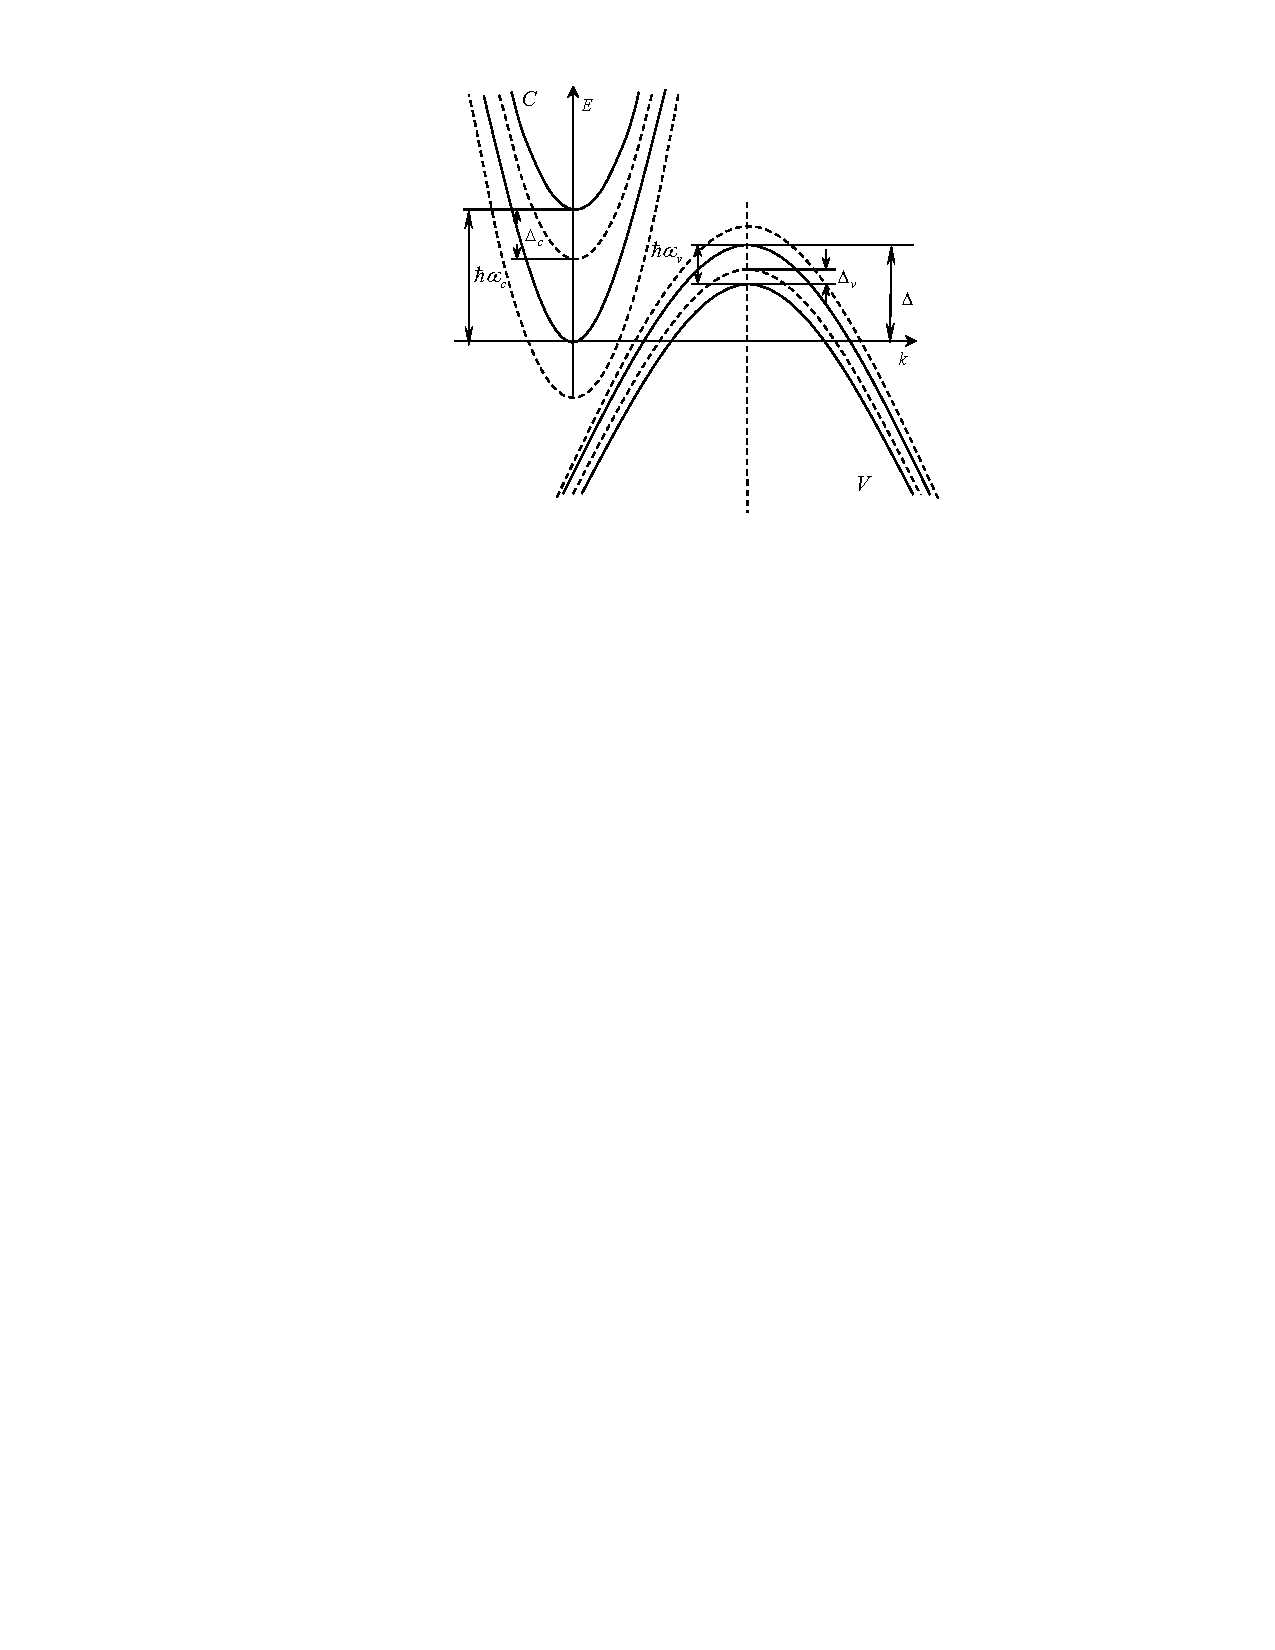
\includegraphics [scale=1.35] {fig_4_4_1}
	\caption{Схема зонной структуры рассматриваемой низкоразмерной системы. Сплошными линиями показаны две нижайшие размерно-квантованные зоны ($c$~---~зоны проводимости, $v$~---~валентные зоны) , пунктирными линиями изображены две нижайшие размерно-квантованные зоны в поперечном электрическом поле; $\xi $~---~химический потенциал.}
	\label{img:fig_4_2_1}
\end{figure}

Далее будем рассматривать квантовую проволоку Bi в простой модели, энергетический спектр которой изображен на рисунке~\ref{img:fig_4_2_1} . Как следует из \eqref{eq:42_10}, с ростом напряженности электрического поля $E$ дно размерно-квантованных c зон опускается на $\Delta_c $ в область запрещенных значений энергии, а экстремумы размерно-квантованных $v$ зон поднимаются вверх на величину $\Delta_v $.

В квантовых проволоках, как следствие одномерности квантовой системы, на дне размерно-квантованных зон возникают особенности в плотности энергетических состояний. Поэтому, если рассматривать случай вырожденного электронного (дырочного) газа, то с ростом $E$ экстремумы, например размерно-квантованных c зон, опускаясь вниз, пересекают химический потенциал, что может приводить к особенностям электропроводности (подвижности) в исследуемой наноструктуре.

Расчет электропроводности проведем так же как в параграфе~\ref{sect4_1} используя время релаксации для рассеяния носителей на шероховатой поверхности в КП в поперечном электрическом поле \eqref{eq:42_50}. Выражение подвижности для электронов и дырок в рассматриваемой модели принимает вид:
\begin{equation} \label{eq:42_60}
	\mu =\frac{\mu_0\sqrt{\pi } }{2\sum_{nm} F(\eta_{nm}^c )} \sum_{nm}\left\{\frac{\ln \left[\exp \left(\eta _{nm}^c \right)+1\right]}{\left(n+m+1+N_c \right)^2 } +\left(\frac{\Delta E_c }{\Delta E_v } \right)\frac{1}{p} \frac{\ln \left[\exp \left(\eta_{nm}^v \right)+1\right]}{\left(n+m+1+N_v \right)^2 } \right\} .
\end{equation}
Здесь введены обозначения:
\[
	\mu_0 =\frac{4R^4 e}{\gamma \Delta E_c } \sqrt{\frac{k_0 T}{2\pi m_c } }, \;
	R=\frac{a}{2}, \;
	N_c =\frac{2\Delta_c }{\hbar \omega_c }, \;
	N_v =\frac{2\Delta_v }{\hbar \omega_v },
\]
\[
	\eta_{nm}^c =\frac{1}{k_0 T} \left[\xi -\hbar \omega_c \left(n+m+1\right)+\Delta_c \right],
\]
\[
	\eta_{nm}^v =\frac{1}{k_0 T} \left[-\xi -\hbar \omega_v \left(n+m+1\right)+\Delta_0 +\Delta_v \right],
\]
\[
	F(\eta_{nm}^c )=\int\limits_0^{\infty }{\frac{dx}{\exp \left(x^2 -\eta_{nm}^c \right)+1}}  ,
\]
$p$~---~число $c$ зон, участвующих в процессах электропроводности. Химический потенциал $\xi $ находится из условия электронейтральности исследуемой наноструктуры (число электронов в зонах проводимости равно числу дырок в валентной зоне)
\begin{equation} \label{eq:42_70}
	p\sqrt{\frac{m_c }{m_v } } \sum_{n,m}\int\limits_{0}^{\infty }{\frac{dx}{\exp \left(x^2 -\eta_{nm}^c \right)+1}}  =
	\sum_{n,m}\int\limits_0^{\infty}{\frac{dx}{\exp \left(x^2 -\eta_{nm}^v \right)+1}}.
\end{equation}
Положение химического потенциала при заданных параметрах наносистемы определяется величиной радиуса $R$ квантовой проволоки и величиной напряженности поперечного электрического поля.

Рассмотрим частные случаи, допускающие аналитическое решение уравнения \eqref{eq:42_70}. Пусть электронный (дырочный) газ является невырожденным. Это возможно, если радиус квантовой проволоки такой, что $\Delta_0 < \hbar \omega_c +\hbar \omega_v $. Как показали экспериментальные исследования \cite{Black2003a} при $R=250 \AA$ в нанопроволоках Bi $\Delta_0 =\hbar \omega_c +\hbar \omega_v $. Если $m_c \ll m_v $ и носители находятся в нижайших размерно-квантованных зонах $(n = m = 0)$, подвижность можно записать в следующем виде:
\begin{equation} \label{eq:42_80}
	\mu =\frac{\mu_0}{\left(1+N_c \right)^2 } .
\end{equation}
Согласно \eqref{eq:42_80} подвижность в рассматриваемом случае с ростом напряженности поперечного электрического поля убывает. Это связано с более сильным взаимодействием носителей с шероховатой поверхностью с увеличением электрического поля.

Если электронный газ вырожден и химический потенциал расположен между нижайшей и последующей размерно-квантованной зоной проводимости (аналогично и для размерно-квантованной v зоны), то подвижность описывается следующим соотношением:
\begin{equation} \label{eq:42_90}
	\mu = \frac{\sqrt{\mu_0 2\pi}}{4\left(1+N_c \right)^2 } \left[\frac{1}{k_0 T} \left(\Delta_0 +\Delta_c +\Delta_v -\hbar \omega_v -\hbar \omega_c \right)\right]^{\frac{1}{2} }
\end{equation}
Как следует из \eqref{eq:42_90}, подвижность с ростом $E$ убывает, но слабее, чем в случае невырожденного электронного газа. В общем случае зависимость подвижности от напряженности поперечного электрического поля можно найти только численно.

\begin{figure}[!h]
	\center
	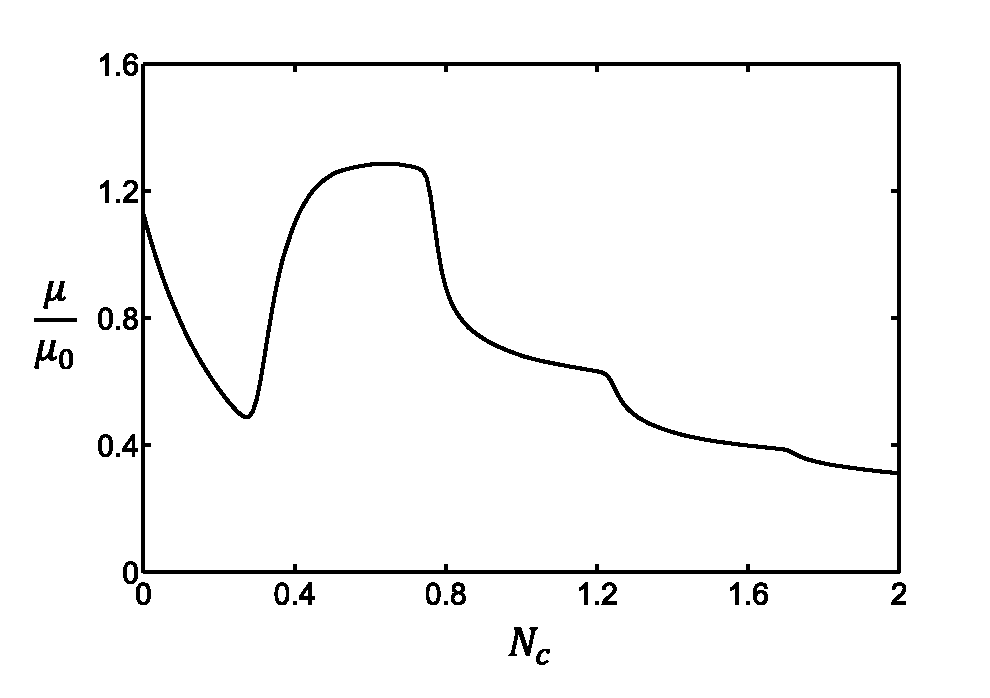
\includegraphics [scale=0.8] {fig_4_2_2}
	\caption{Зависимость подвижности (в относительных единицах) от напряженности поперечного электрического поля. $R=330 \AA$.}
	\label{img:fig_4_2_2}
\end{figure}

\begin{figure}[!h]
	\center
	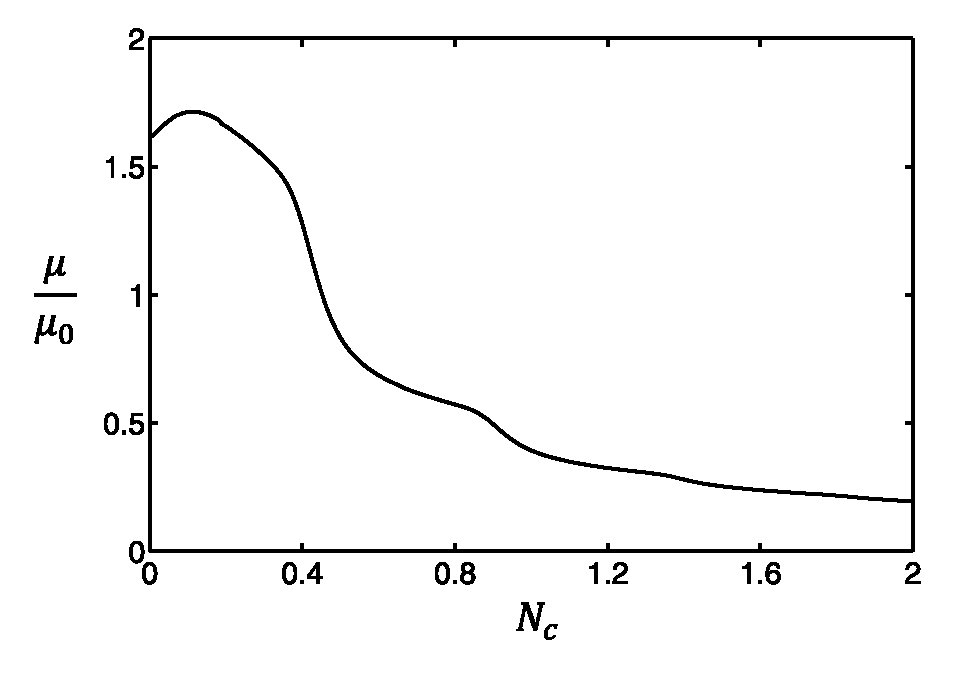
\includegraphics [scale=0.8] {fig_4_2_3}
	\caption{Зависимость подвижности (в относительных единицах) от напряженности поперечного электрического поля. $R=990 \AA$.}
	\label{img:fig_4_2_3}
\end{figure}

Влияние поперечного электрического поля на подвижность принципиальным образом зависит от радиуса нанопроволоки. При небольших значениях $R$, когда квантовая проволока представляет почти безщелевой полупроводник, с ростом $E$ (при $E=0$ электронный (дырочный) газ невырожден) подвижность сначала уменьшается (см формулу \eqref{eq:42_80}), затем увеличивается, и в дальнейшем описывается осцилляционной кривой (рисунок~\ref{img:fig_4_2_2}). При больших радиусах нанопроволок, когда электронный (дырочный) газ изначально был вырожден, зависимость $\mu$ от $E$ носит явно осциллирующий характер (рисунок~\ref{img:fig_4_2_3}). Такое поведение подвижности в присуствии поперечного электрического поля связано с тем, что с ростом напряженности поперечного электрического поля, дно размерно-квантованных $c$ зоны, опускаясь в область запрещенных значений энергии, пересекает химический потенциал, что приводит к увеличению подвижности. Заметим, что для типичных значений параметров нанопроволок Bi ($m_c = 0.01m_0 $, $m_v = 0.1m_0$, $\Delta E_c  / \Delta E_v  = 1.5$) $N_v =5.8 N_c $, поэтому с ростом $E$ влияние дырок на поведение $\mu$ от $E$ слабее, чем для электронов. Следовательно, осцилляционная зависимость подвижности от $E$ (рисунок~\ref{img:fig_4_2_3}) должна наблюдаться и для полупроводниковых квантовых проволок с вырожденным электронным газом.

\section{Особенности подвижности в нанопроволоках в поперечных электрическом и магнитном полях} \label{sect4_3}
В присутствии однородного квантующего магнитного поля энергетический спектр носителей в квантовых проволоках заметным образом меняется, поэтому рассмотрим одновременное влияние поперечного магнитного и электрического полей $(\vect{B}\parallel\vect{E})$ на явления переноса в квантовых проволоках. Время релаксации с учетом анизотропии эффективных масс носителей в такой системе определяется выражением \eqref{eq:1_20}. Матричный элемент импульса \footnote{Недиагональные по осцилляторному квантовом числу матричные элементы оператора импульса при разумных параметрах КП дают незначительный вклад в искомую электропроводность}:
\[
	\hat{P}^{(x)}_{\alpha \beta }=\hbar k_x{\left(\frac{\omega_y}{\Omega_y}\right)}^2 \delta_{\alpha \beta }.
\]
В этих естественных приближениях соотношение для электропроводности \eqref{eq:31_150} с учетом  \eqref{eq:1_20}, после интегрирования по $k_x$, можно записать в следующем виде:
\begin{equation} \label{eq:43_60}
	\sigma_{xx}=\frac{2 e^2\hbar}{\beta_0 \pi^2 m^*_x \gamma_0} \sum_{nm}{\frac{\ln \left[1+\exp\left(\beta_0 \xi_{nm}\right)\right]}{\left[\hbar \omega_y \frac{\omega_y}{\Omega_y}\left(n+\frac{1}{2}\right)+\hbar \omega_z\left(m+\frac{1}{2}\right)+2\Delta_c\right]^2}}
\end{equation}
\[
	\xi_{nm}=\xi -\hbar \Omega_y \left(n+\frac{1}{2}\right)-\hbar \omega_z\left(m+\frac{1}{2}\right)+\Delta_c,\;
	\beta =\frac{1}{k_0 T}
\]
$\xi $~---~химический потенциал исследуемой наносистемы. Аналогично можно записать $\sigma_{xx}$ для дырок в валентной зоне полуметалла Bi. В этом случае в \eqref{eq:43_60} эффективные массы электронов нужно заменить на соответствующие массы дырок $\mu_x,\; \mu_y,\; \mu_z$, а $\xi$  на $-\xi +\Delta_0$ ($\Delta_0$ определяется перекрыванием валентной зоны и зоны проводимости, $\Delta_0\cong 39\text{ meV}$ \cite{Levin2009a}).

Энергия электронов в валентной зоне определяется соотношением:
\[
	E^v_{\alpha }={\Delta }_0-\frac{{\hbar }^2k^2_x}{2{\mu }^*_x}-\hbar {\widetilde{\Omega }}_y\left(n+\frac{1}{2}\right)-\hbar {\widetilde{\omega }}_z\left(m+\frac{1}{2}\right)+{\Delta }_v,
\]
здесь обозначено
\[
	\widetilde{\omega}_i=\frac{1}{R}{\left[\frac{2 \Delta E_v}{\mu_i}\right]}^{\frac{1}{2}},\;
	{\widetilde{\Omega }}^2_y=\frac{\mu_x}{\mu_y}{\left({\widetilde{\omega }}^c_x\right)}^2+{\widetilde{\omega }}^2_y,\ \ {\widetilde{\omega }}^c_x=\frac{eH}{{\mu }_xc},\;
\]
\[
	\mu^*_x=\mu_x{\left(\frac{\widetilde{\Omega}_y}{\widetilde{\omega}_y}\right)}^2,\;
	\Delta_v = \frac{{\left(eER\right)}^2}{4\Delta E_v},
\]
$\hbar {\widetilde{\Omega }}_y, \hbar {\widetilde{\omega }}_z$ -- энергия размерного квантования в валентной зоне, $\Delta E_v$ -- высота потенциальной энергии для дырок на границе квантовой проволоки.

Следовательно, подвижность носителей (электронов и дырок) в нанопроволоке записывается следующим образом:
\begin{multline} \label{eq:43_70}
	\mu =\frac{eR^2{\hbar }^2}{m^*_x \gamma_0}\frac{1}{\sqrt{2m^*_x \beta_0}\sum_{nm}{F\left(\xi_{nm}\right)}}\sum_{nm}{\frac{\ln \left[1+{\exp \left(\beta {\xi }_{nm}\right)\ }\right]}{\left[\hbar \omega_y\frac{\omega_y}{\Omega_y} \left(n+\frac{1}{2}\right)+\hbar \omega_z\left(m+\frac{1}{2}\right)+ 2\Delta_c\right]^2}}+\\
	+\frac{eR^2 \hbar^2}{\mu^*_x \gamma_0}\frac{1}{\sqrt{2\mu^*_x \beta_0}\sum_{nm}{F\left(\widetilde{\xi }_{nm}\right)}}\sum_{nm}{\frac{\ln \left[1+{\exp \left(\beta \widetilde{\xi}_{nm}\right)\ }\right]}{p{\left[\hbar \widetilde{\omega}_y \frac{\widetilde{\omega}_y}{\widetilde{\Omega}_y}\left(n+\frac{1}{2}\right)+\hbar \widetilde{\omega}_z \left(m+\frac{1}{2}\right)+2{\Delta }_v\right]}^2}}
\end{multline}
\[
	F\left(\xi_{nm}\right)=\int\limits^{\infty }_0 {\frac{dx}{\exp \left(x^2-\beta {\xi }_{nm}\right) +1}},
\]
\[
	\widetilde{\xi }_{nm}=-\xi -\hbar \widetilde{\Omega}_y\left(n+\frac{1}{2}\right)-\hbar \widetilde{\omega}_z\left(m+\frac{1}{2}\right)+\Delta_0+\Delta_v
\]
$p$~---~число $c$ зон, участвующих в процессах электропроводности. Если магнитное поле направлено вдоль оси OZ, а постоянное поперечное электрическое поле $\vect{E}$ перпендикулярно $\vect{H}$, то подвижность, как показывают расчеты, тоже описывается соотношением \eqref{eq:43_70}.

Химический потенциал $\xi $ находится из условия электронейтральности исследуемой квантовой проволоки (число электронов в $p$ зонах проводимости равно числу дырок в валентной зоне):
\begin{equation} \label{eq:43_80}
	p{\left(\frac{m^*_x}{{\mu }^*_x}\right)}^{\frac{1}{2}}\sum_{nm}{F\left({\xi }_{nm}\right)}=\sum_{nm}{F\left({\widetilde{\xi }}_{nm}\right)}
\end{equation}
Из \eqref{eq:43_80} следует что, величина химического потенциала $\xi $ зависит от радиуса нанопроволоки и определяется напряженностью электрического и магнитного полей.

Дальнейшие оценки будем проводить для параметров, близких к полуметалу Bi: $m_x=0.0011m_0$, $m_y=0.26m_0$, $m_z=0.0045m_0$, ${\mu }_x={\mu }_y= 0.059 m_0$, $\mu_z = 0.634$ \cite{Levin2009a}, $\Delta E_c=0.5\text{ eV}$, $\Delta E_v =0.3\text{ eV}$ ($m_0$~---~масса свободного электрона). При этих параметрах
\[
	\hbar {\omega }_y=\frac{4.9}{R_0}\left(eV\right),\;
	\hbar {\omega }_z=\frac{37.6}{R_0}\left(eV\right),\;
	\hbar {\widetilde{\omega }}_y=\frac{8}{R_0}\left(eV\right),\;
	\hbar {\widetilde{\omega }}_z=\frac{2.4}{R_0}\left(eV\right),
\]
($R_0$~---~радиус нанопроволоки в ангстремах).

\begin{figure}[!h]
	\center
	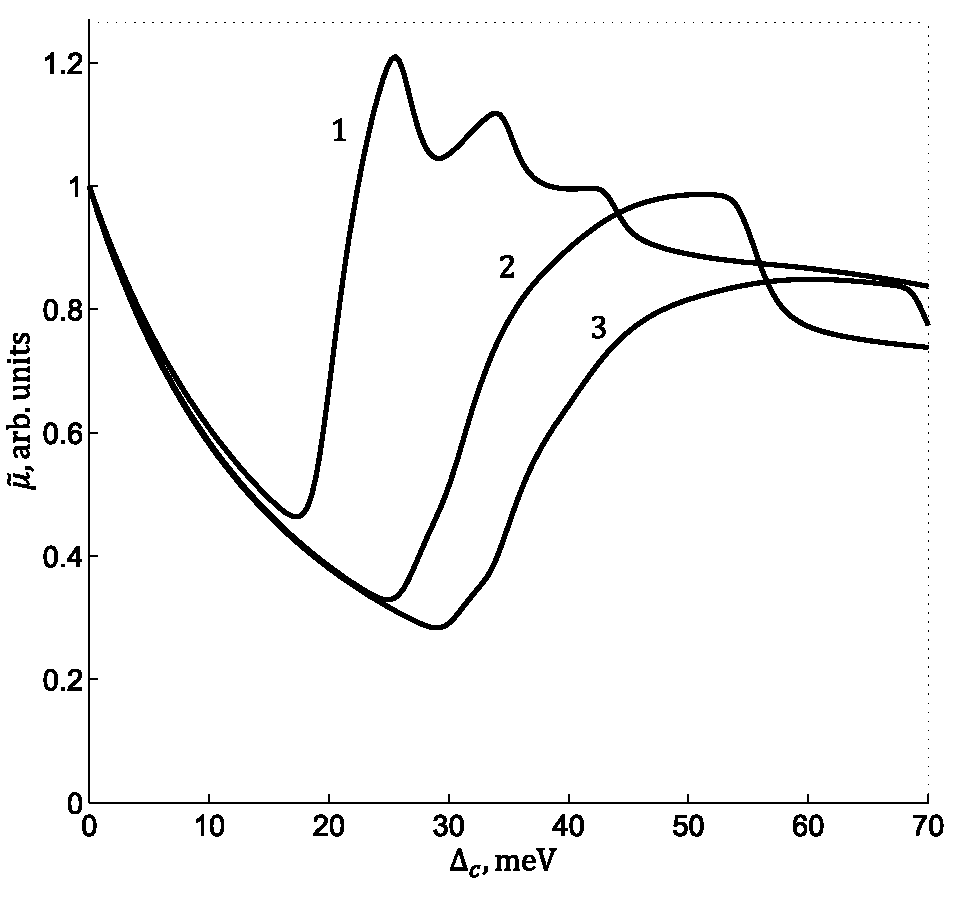
\includegraphics [scale=0.8] {fig_4_3_1}
	\caption{Зависимость подвижности в относительных единицах $\widetilde{\mu}=\mu(E)/\mu(0)$ от электрического поля.}
	\label{img:fig_4_3_2}
\end{figure}

На рисунке~\ref{img:fig_4_3_2} приведены численные расчеты зависимости подвижности (в относительных единицах) от напряженности поперечного электрического поля. Кривые 1, 2, 3 получены при $\delta = 0$, $\delta = 0.05$, $\delta = 0.1$ соотвественно $\left(\delta = {\left(\omega^c_x/\omega_y\right)}^2\right)$. При малых значениях $\Delta_c$ электронный газ (при рассмотренных параметрах квантовой проволоки) является невырожденным, поэтому с ростом напряженности поперечного электрического поля подвижность уменьшается \eqref{eq:42_80}. Кривая 1 (подвижность в отсутствии  магнитного поля $\delta = 0$) описывается тремя максимумами. Такая осцилляционная зависимость подвижности связана с тем, что с ростом $E$ химический потенциал, отсчитанный от дна размерно-квантованной зоны проводимости, поднимается в область больших значений энергии и может пересечь дно размерно-квантованной $c$ зоны, в которой существуют особенности в плотности энергетических состояний. Первый пик связан с пересечением химического потенциала нижайшего состояния размерно-квантованной $c$ зоны $(n=0,\; m=0)$, второй пик возникает из-за пересечения химического потенциала дна первой размерно-квантованной зоны $(m=0,\; n=1)$, третий пик -- из-за пересечения химического потенциала второй размерно-квантованной зоной $(m=1,\; n=0)$. С ростом напряженности магнитного поля дно размерно-квантованной зоны проводимости поднимается в область больших значений энергии, поэтому пересечение химического потенциала наступает при больших значениях $\Delta_c$. Именно по этой причине первый пик кривой 2 сдвинут по отношению первого пика кривой 1 в область больших значений напряженности поперечного электрического поля.

Заметим, что согласно \eqref{eq:43_70} подвижность с ростом напряженности магнитного поля уменьшается. Это связано с тем, что эффективные массы электронов (дырок) в однородном поперечном магнитном поле увеличиваются (в ${\left(\Omega_y /\omega_y\right)}^2$ раз для электронов и в ${\left({\widetilde{\Omega }}_y/{\widetilde{\omega }_y}\right)}^2$ раз для дырок).

\section{Термоэдс в нанопроволоках Bi в попереченом постоянном электрическом поле}\label{sect4_4}

Исследования термомагнитных явлений в объемных материалах в поперечном магнитном поле представляются очень важными, поскольку квантовые эффекты в этом случае проявляются очень ярко. Именно по этой причине описание кинетических явлений с использованием классического уравнения Больцмана, которое неприменимо в квантующих магнитных полях, является сомнительным \cite{Askerov1970}. В массивных образцах в поперечном магнитном поле термоэдс простым образом связана с потоком тепловой энергии $\gamma_{\alpha\beta}$ и с электропроводностью $\sigma_{\alpha\beta}$ (принцип Онзагера)
\[
	\alpha_{xx}(H) = \frac{\gamma_{yx}}{T \sigma_{yx}}
\]
и при $\omega_c \tau \gg 1$ ($\omega_c$~---~циклотронная частота, $\tau$~---~время релаксации) не зависит от механизма рассеяния \cite{Askerov1970}. В низкоразмерных системах термоэдс в поперечном магнитном поле принципиальным образом отличается от массивных образцов. Это связано с тем, что диагональные по квантовым числам матричные элементы операторов плотности электрического тока, через которые определяются корреляционные функции плотности потока тепловой энергии и электропроводности, отличны от нуля. Поэтому термоэдс в рассматриваемом случае
\begin{equation} \label{eq:44_05}
	\alpha_{xx}(H) = \frac{\gamma_{xx}}{T \sigma_{xx}}
\end{equation}
и зависит от механизмов рассеяния носителей в системах с пониженной размерностью (квантовые ямы, квантовые проволоки). Для последовательного описания термоэдс в поперечном квантующем магнитном поле в дальнейшем используются общие соотношения неравновесной квантовой статистики для потока тепловой энергии и электропроводности \cite{Kubo1957}, расчет которых можно провести без использования решения классического уравнения Больцмана \cite{Khamidullin2002}. Усреднение по фононной подсистеме и усреднение по реализации случайного процесса при учете рассеяния носителей на шероховатой поверхности проводится с использованием метода кумулянтного усреднения (глава~\ref{chapt3}). В результате:
\begin{equation} \label{eq:44_07}
	\gamma_{xx} = \int\limits_{- \infty }^{\infty}{\left\langle \hat{j_x}(t) \hat{Q}_x \right\rangle  dt} =
	\frac{\beta e \hbar^2 }{2 k_0 TV m_e^2} \sum_{\alpha}{\left( E_{\alpha} - \xi \right) k_x^2 \tau_{\alpha} n_{\alpha}\left( 1 - n_{\alpha} \right) }
\end{equation}
\begin{equation} \label{eq:44_08}
	\sigma_{xx} = \int\limits_{- \infty }^{\infty}{\left\langle \hat{j}_x(t) \hat{j}_x \right\rangle  dt} =
	\frac{\beta e^2 \hbar^2 }{2 k_0 T V m_e^2} \sum_{\alpha}{k_x^2 \tau_{\alpha} n_{\alpha}\left( 1 - n_{\alpha} \right) }
\end{equation}
$n_{\alpha}$~---~равновесная функция распределения носителей, $\alpha$~---~набор квантовых чисел, описывающих квантовое состояние электрона, $1/\tau_{\alpha}$~---~полная квантово-механическая вероятность рассеяния частиц в единицу времени, $\xi$~---~химический потенциал, $k_x$~---~волновой вектор вдоль оси OX для электрона с эффективной массой $m_e$, $\left\langle \cdots \right\rangle$~---~описывает усреднение с равновесной матрицей плотности.

Именно примененный в диссертации метод расчета термоэдс, не использующий классическое кинетическое уравнение Больцмана, позволяет последовательно рассматривать квантующие магнитные поля, а также учитывать корневые особенности в плотности состояний на дне размерно-квантованной зоны, возникающие в одномерных системах.

В квантовых проволоках, как следствие одномерности исследуемой наносистемы, на дне размерно-квантованных зон возникают особенности в плотности энергетических состояний. Это обстоятельство приводит, в частности, к особенностям оптических свойств нанопроволок \cite{Black2003a,Black2000,Black2002,Levin2009a}, и заметным образом влияет, как будет показано ниже, на кинетические коэффициенты в нанопроволоках с вырожденным электронным (дырочным) газом. В этом параграфе диссертационной работы теоретически исследуется термоэдс в квантовых проволоках типа Bi в модели квадратичного потенциала. Если постоянное электрическое поле $E$, направленное вдоль оси размерного квантования наноструктуры, при определенных условиях может существенным образом влиять на подвижность как показано в параграфе \ref{sect4_3}, то представляет интерес исследовать влияние $E$ на термоэдс в низкоразмерных системах.

В квантовых проволоках типа Bi с потенциальной энергией для носителей в форме параболоида вращения в постоянном электрическом поле $E$, направленном перпендикулярно оси исследуемой наноструктуры энергия электронов с эффективной массой $m_e $ в размерно-квантованной зоне проводимости и дырок с эффективной массой $m_h$ в валентной зоне имеют вид \eqref{eq:42_10}.

Как следует из \eqref{eq:42_10} с ростом напряженности электрического поля дно размерно-квантованной зоны проводимости опускается в запрещенную зону. Именно это обстоятельство приводит к тому, что при учете рассеяния электронов на шероховатой поверхности время релаксации зависит от $E$, что и приводит к заметному изменению кинетических коэффициентов (глава~\ref{chapt3}). С ростом $E$ носители «прижимаются» к поверхности наноструктуры, т.е. их взаимодействие с шероховатой поверхностью увеличивается, что приводит к уменьшению времени релаксации.

Далее для нанопроволок Bi рассмотрим простейшую модель перекрывающихся зон (рисунок~\ref{img:fig_4_2_1}). На рисунке~\ref{img:fig_4_2_1} сплошными линиями изображены  размерно-квантованные уровни c и v зон. Пунктирными линиями представлены энергии носителей в постоянном электрическом поле.

Расчет термоэдс $\alpha_{xx} $ (слабое тянущее электрическое поле направленно вдоль оси x) проводился с использованием общих соотношений, связывающих $\alpha_{xx} $ с плотностью потока тепловой энергии $\gamma_{xx} $ для носителей и с электропроводностью для электронов и дырок \cite{Kubo1957}.

Аналогично \eqref{eq:44_07}, \eqref{eq:44_08} записывается $\sigma_{xx}^{(h)} $, $\gamma_{xx}^{(h)} $ для дырок в $v$ зоне:
\begin{equation} \label{eq:44_31_01}
	\sigma_{xx}^{(h)} =\frac{\beta e^2 \hbar^2 }{2V m_v^2 } \sum_{\alpha }k_x^2 \tau_{\alpha }^{(h)} n^{(h)}_{\alpha } \left(1-n^{(h)}_{\alpha } \right),
\end{equation}
\begin{equation} \label{eq:44_31}
	\gamma_{xx}^{(h)} =\frac{\beta e^2 \hbar^2 }{2 V m_v^2 } \sum _{\alpha }\left(E_{\alpha }^{(h)} -\xi \right)k_x^2 \tau _{\alpha }^{(h)} n^{(h)}_{\alpha } \left(1-n^{(h)}_{\alpha } \right) ,
\end{equation}
Время релаксации $\tau_\alpha $ при рассеянии носителей на $\delta $-образной шероховатой поверхности определялось ранее \eqref{eq:42_50}. Аналогично записывается $\tau_{\alpha }^{(h)} $ для дырок.
\begin{equation} \label{eq:44_40}
	\frac{1}{\tau_{\alpha }^{(h)} } =\frac{2m_v \omega_v^2 \gamma_0^{(h)} }{\hbar R^2 \left| k_x \right|} \left[n+m+1+N_v \right]^2, \; N_v =\frac{2 \Delta_v }{\hbar \omega_v} ,
\end{equation}

В результате выражение для термоэдс после суммирования по $k_x $ принимает вид:
\begin{multline} \label{eq:44_50}
	\alpha _{xx} =-\frac{k_0}{e} \left\{\sum_{n,m}\left[\nu \frac{F_2 \left(\eta_{nm}^c \right)-\eta _{nm}^c F_1 \left(\eta_{nm}^c \right)}{\left(n+m+1+N_c \right)^2 } -\frac{F_2 \left(\eta_{nm}^v \right)-\eta_{nm}^v F_1 \left(\eta_{nm}^v \right)}{b\left(n+m+1+aN_c \right)^2 } \right] \right\}\times\\
	\times \left\{\sum _{n,m}\left[\nu \frac{F_1 \left(\eta_{nm}^c \right)}{\left(n+m+1+N_c \right)^2 } +\frac{F_1 \left(\eta_{nm}^v \right)}{b\left(n+m+1+a N_c \right)^2 } \right] \right\}^{-1}
\end{multline}
\[
	a=\left(\frac{m_h }{m_c } \right)^{\frac{1}{2} } \left(\frac{\Delta E_c }{\Delta E_v } \right)^{\frac{3}{2} } ,\;
	b=\frac{\Delta E_v }{\Delta E_c } ,
\]
\[
	\eta_{nm}^c =\beta \left[\Delta_c +\xi -\hbar \omega_c \left(n+m+1\right)\right],
\]
\[
	\eta_{nm}^v =\beta \left[\Delta +\Delta_v -\xi -\hbar \omega_v \left(n+m+1\right)\right],
\]
$v$~---~количество зон проводимости, участвующих в кинетических процессах,
\begin{equation} \label{eq:44_55}
	F_k (\eta )=\int\limits_0^{\infty }{\frac{ e^{x-\eta } x^k dx}{\left(1 + e^{x-\eta }\right)^2 }} ,
\end{equation}
функция \eqref{eq:44_55} выражается через интегралы Ферми, определяемые как \cite{Dingle1957,Blakemore1982}
\[
	\mathcal{F}_j (\eta )=\frac{1}{\Gamma(j+1)}\int\limits_0^{\infty }{\frac{x^j dx}{\left(1 + e^{x-\eta }\right) }} ,
\]
следующим образом \cite{Askerov1970}:
\[
	F_k (\eta ) =k \Gamma(k) \mathcal{F}_{k-1} (\eta ).
\]
Для $k=1$ выражение \eqref{eq:44_55} записывается в элементарных функциях \cite{Rhodes1950}:
\[
	F_1 (\eta )=\ln \left(1 + e^{\eta }\right)
\]
Химический потенциал $\xi $ определяется как обычно из условия электронейтральности исследуемой наноструктуры (число электронов в размерно-квантованных $c$ зонах равно числу дырок в $v$ зоне):
\begin{equation} \label{eq:44_60}
	\nu \sqrt{\frac{m_e }{m_v } } \sum_{n,m}F_{\frac{1}{2}}\left(\eta_{nm}^c \right) =\sum_{n,m}F_{ \frac{1}{2}} \left(\eta_{nm}^v \right) .
\end{equation}
Аналитическое решение уравнения \eqref{eq:44_60} для химического потенциала можно найти для частных случаев.

Если носители находятся на нижайшем размерно-квантованном уровне $(n=m=0)$, электронный и дырочный газ вырожден (химический потенциал положителен и $\beta \xi \gg 1$), то при $m_c \ll m_v $, из \eqref{eq:44_60} не трудно определить $\xi $:
\[
	\xi -\hbar \omega_c =\Delta_0 +\Delta_v -\left(\hbar \omega_c +\hbar \omega_v \right), \left(\frac{\Delta_v }{\Delta_c } =\frac{\Delta E_c }{\Delta E_v } >1\right).
\]
$\xi -\hbar \omega_c $~---~химический потенциал отсчитываемый от дна размерно-квантованной зоны проводимости.

В такой простой модели, термоэдс принимает вид:
\begin{equation} \label{eq:44_70}
	\alpha_{xx}^{(d)} =-\frac{k_0 }{e} \cdot \frac{\pi^3}{3} \cdot \frac{1-\frac{1}{b\nu } \left(\frac{1+N_c }{1+aN_c } \right)^2 }{\Delta +\Delta_v -\left(\hbar \omega_c +\hbar \omega_v \right)} .
\end{equation}
Следовательно, термоэдс отрицательна, т.е. определяется электронами и с ростом напряженности электрического поля $E$ уменьшается.

В противоположном случае невырожденного электронного и дырочного газов (это справедливо при малых радиусах квантовой проволоки $d \ll 500 \AA$, при $T=77 \text{ K}$ \cite{Black2002}), как следует из уравнения \eqref{eq:44_60}, химический потенциал определяется из соотношения:
\begin{equation} \label{eq:44_80}
	\nu \sqrt{\frac{m_c }{m_v } } \exp \left(\eta_{00}^c \right)=\exp \left(\eta_{00}^v \right).
\end{equation}
В результате
\begin{equation} \label{eq:44_90}
	\alpha_{xx}^{(nd)} =-\frac{k_0 }{e} \left\{2+\beta \left[\frac{1}{2} \ln \left( \nu^2 \frac{m_e }{m_h } \right) +\left(\hbar \omega_c +\hbar \omega_v -\Delta +\Delta_v +\Delta_c \right)\right]\right\},
\end{equation}

\begin{figure}[!h]
	\center
	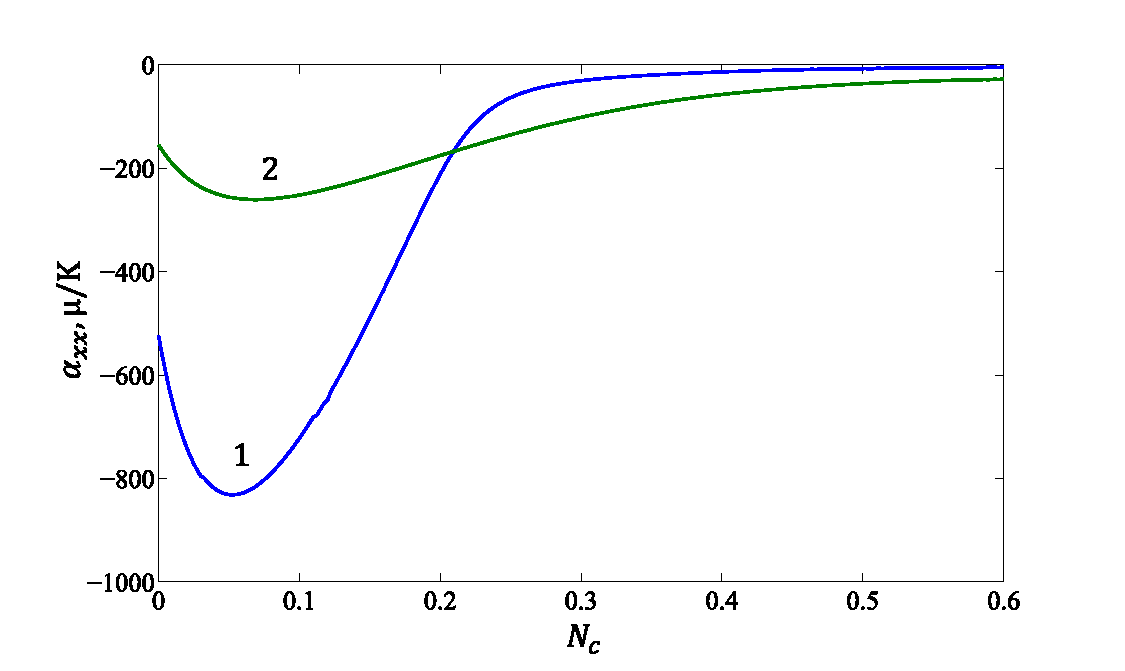
\includegraphics [scale=0.8] {fig_4_4_2}
	\caption{Зависимость удельной термоэдс квантовой проволоки от напряженности поперечного электрического поля}
	\label{img:fig_4_4_2}
\end{figure}

Расчет термоэдс в общем случае проведен по соотношению \eqref{eq:44_50} с учетом размерно-квантованных v и c зон при типичных значениях параметров квантовой проволоки: $\Delta E_c =0.5 \text{ eV}$, $\Delta E_v =0.3 \text{ eV}$, $\Delta_0 =0.038 \text{ eV}$, $m_c =0.01 m_0 $, $m_v = 0.1m_0 $, при $R=500 \AA$. Зависимость термоэдс от напряженности постоянного электрического поля приведена на рисунке~\ref{img:fig_4_4_2}.

Кривая 1 получена при $T=10 \text{ K}$, кривая 2 вычислена при $T=50 \text{ K}$. Как показано на рисунке~\ref{img:fig_4_4_2} с ростом температуры величина термоэдс по абсолютной величине уменьшается и при увеличении $E$, стремится к нулю оставаясь при этом отрицательной.

В нанопроволоках, как следствие одномерности наноструктуры в плотности состояний на дне каждой размерно-квантованной зоны возникают особенности. Поэтому с ростом напряженности постоянного электрического поля экстремумы, например, размерно-квантованных $v$ зон, поднимаясь вверх по энергии, могут пересекать химический потенциал, что, естественно, приводит к особенностям кинетических коэффициентов (например, подвижности). Однако в термоэдс эти особенности не очень ярко проявляются, поскольку $\alpha _{xx} $ определяется отношением потока тепловой энергии носителей к электропроводности.

При $E=0$ дырки вносят заметный вклад в термоэдс, уменьшая ее по абсолютной величине. С ростом напряженности электрического поля (для рассмотренных выше параметров нанопроволоки $a\sim 7$) вклад дырок в термоэдс быстро уменьшается, а это и приводит к тому, что в зависимости $\alpha_{xx} $ от $N_c $ (рисунок~\ref{img:fig_4_4_2}) возникает характерный минимум.

Следовательно, внешнее электрическое поле дает уникальную возможность управлять величиной термоэдс, что позволяет надеяться  на приборное применение предсказанного эффекта. В заключение отметим, что сильная анизотропия эффективных масс в нанопроволоках Bi (в зависимости от направления кристаллографических осей массы для электронов в $c$-зоне меняются от $0,001 m_0 $ до $0,26 m_0 $, в валентной зоне от $0,059m_0 $ до $0,634m_0 $ \cite{Levin2009a}) влияет на величину рассматриваемого эффекта, но сохраняет зависимость термоэдс от $E$ практически неизменной.
